% !TeX encoding = UTF-8
% !TeX spellcheck = pl_PL

% $Id:$





\newcommand{\kurs}{Wizualizacja danych sensorycznych}
\newcommand{\formakursu}{Projekt}


\newcommand{\doctype}{Raport ze wczesnego etapu projektu}




\newcommand{\projectname}{Wizualizacja warunk\'{o}w narciarskich w g\'{o}rach}






\newcommand{\osobaA}{Wojciech \textsc{Kosicki}, 234506}


\newcommand{\termin}{cz 18:55}


\newcommand{\prowadzacy}{Dr in\.{z}. Bogdan \textsc{Kreczmer}}

\documentclass[10pt, a4paper]{article}


%Preambuła dokumentu

% linki w spisie tresci, bibliografi
\usepackage[bookmarks=true,bookmarksnumbered=false,unicode=true,pdftex=true, colorlinks,filecolor=black,linkcolor=black,urlcolor=black,citecolor=black]{hyperref}

%ustawienie rozmiaru papieru
\usepackage[a4paper, left=2.5cm, right=2.5cm, top=2.5cm, bottom=2.5cm, headsep=1.2cm]{geometry}

%rozmaite ustawienia pozwalające okreslić język

%NALEŻY wybrać jeden z pakietów
%\usepackage{polski} %przydatne podczas składania dokumentów w j. polskim
\usepackage[polish]{babel}  % pakiet lokalizujący dokument w języku polskim
%\usepackage[british]{babel}

\usepackage{indentfirst}	% polski styl pisania (np. rozpoczecie pierwszego akapitu
% pod nazwa rozdzialu od wciecia)
%\usepackage[OT4]{fontenc}
\usepackage[utf8]{inputenc} % w miejsce utf8 można wpisać latin2 bądź cp1250,
% w zależności od tego w jaki sposób kodowane są 
% polskie znaki diakrytyczne przy wprowadzaniu 
% z klawiatury.
%kodowanie znaków, zależne od systemu
\usepackage[T1]{fontenc} %poprawne składanie polskich czcionek

%OPEROWANIE NA OBRAZACH
\usepackage{graphicx}       % pakiet graficzny, umożliwiający m.in.
% import grafik w formacie eps
%\usepackage{epstopdf}		% pozwala na importowanie grafik w formacie eps
% przy użyciu pdflatex
\usepackage[update,prepend]{epstopdf}
\usepackage{rotating}       % pakiet umożliwiający obracanie rysunków
\usepackage{subfigure}      % pakiet umożliwiający tworzenie podrysunków
\usepackage{epic}           % pakiet umożliwiający rysowanie w środowisku latex
\usepackage{psfrag}         % pakiet umożliwiający podmianę łańcuchów znaków 
% w plikach eps
%\usepackage{curves}         % pakiet do wykreslania krzywych

%pakiety dodające dużo dodatkowych poleceń matematycznych
\usepackage{amsfonts}       % pakiet z rozmaitymi czcionkami matematycznymi
%\usepackage{amssymb}        % pakiet z rozmaitymi symbolami matematycznymi
\usepackage{amsmath}        % pakiet z rozmaitymi środowiskami matematycznymi

\usepackage{fp}             % pakiet z funkcjami operujacymi 
% na liczbach zmiennoprzecinkowych
\usepackage{calc}           % pakiet umożliwiający operacje arytmetyczne
% na tzw. licznikach (liczbach całkowitych)
\usepackage{leftidx}		% indeksy górne i dolne po lewej stronie

%definicje matematyczne
\providecommand{\abs}[1]{\lvert#1\rvert}
\providecommand{\norm}[1]{\lVert#1\rVert}

%pakiety wspomagające i poprawiające składanie tabel
\usepackage{supertabular}
\usepackage{array}
\usepackage{tabularx}
\usepackage{hhline}
\usepackage{longtable}		% wsparcie dla dlugich tabel
\usepackage{multicol}		% podzial strony na wiele kolumn

%pakiet do BibTex
\usepackage{cite}

\usepackage{url} %pakiet pozawalający na dodawanie adresów url w bibliografi

%pakiet wypisujący na marginesie etykiety równań i rysunków zdefiniowanych przez \label{}, chcąc wygenerować finalną wersję dokumentu wystarczy usunąć poniższą linię
%\usepackage{showlabels}

\usepackage{float}			% lepsza obsluga mechanizmow obiektow plywajacych
% wymuszenie wstawienia np. tabeli, obrazka w danym miejscu przez [H]

\usepackage{listings}       % pakiet dedykowany zrodlom programow
\usepackage{color}


\definecolor{dkgreen}{rgb}{0,0.6,0}
\definecolor{gray}{rgb}{0.5,0.5,0.5}
\definecolor{mauve}{rgb}{0.58,0,0.82}

\lstset{ %
	language=Matlab,                % the language of the code
	basicstyle=\scriptsize,           % the size of the fonts that are used for the code
	numbers=left,                   % where to put the line-numbers
	numberstyle=\tiny\color{gray},  % the style that is used for the line-numbers
	stepnumber=1,                   % the step between two line-numbers. If it's 1, each line 
	% will be numbered
	numbersep=5pt,                  % how far the line-numbers are from the code
	backgroundcolor=\color{white},      % choose the background color. You must add \usepackage{color}
	showspaces=false,               % show spaces adding particular underscores
	showstringspaces=false,         % underline spaces within strings
	showtabs=false,                 % show tabs within strings adding particular underscores
	%frame=single,                   % adds a frame around the code
	rulecolor=\color{black},        % if not set, the frame-color may be changed on line-breaks within not-black text (e.g. comments (green here))
	tabsize=2,                      % sets default tabsize to 2 spaces
	captionpos=b,                   % sets the caption-position to bottom
	breaklines=true,                % sets automatic line breaking
	breakatwhitespace=false,        % sets if automatic breaks should only happen at whitespace
	%title=\lstname,                   % show the filename of files included with \lstinputlisting;
	% also try caption instead of title
	keywordstyle=\color{blue},          % keyword style
	commentstyle=\color{dkgreen},       % comment style
	stringstyle=\color{mauve},         % string literal style
	escapeinside={\%*}{*)},            % if you want to add LaTeX within your code
	morekeywords={*,...},              % if you want to add more keywords to the set
	deletekeywords={...}              % if you want to delete keywords from the given language
}

%polish signs in lst code
\lstset{literate=%
	{ą}{{\k{a}}}1
	{ć}{{\'c}}1
	{ę}{{\k{e}}}1
	{ł}{{\l}}1
	{ń}{{\'n}}1
	{ó}{{\'o}}1
	{ś}{{\'s}}1
	{ż}{{\.z}}1
	{ź}{{\'z}}1
	{Ą}{{\k{A}}}1
	{Ć}{{\'C}}1
	{Ę}{{\k{E}}}1
	{Ł}{{\L}}1
	{Ń}{{\'N}}1
	{Ó}{{\'O}}1
	{Ś}{{\'S}}1
	{Ż}{{\.Z}}1
	{Ź}{{\'Z}}1
}

\usepackage{verbatim}       % pakiet dedykowany rozmaitym wydrukom tekstowym
\usepackage{ifthen}         % pakiet umożliwiający tworzenie prostych programów
% (m.in. zawiera instrukcje powtórzeniowe 
% i warunkowe)
\usepackage{upquote}		%normal quotations marks ' and `

% deklaracje wymagane przez pakiet theorem automatycznie ladowany w przypadku
% klasy dokumentu article
%
\newtheorem{Dn}{Definicja}[section]     % deklaracja srodowiska definicja
\newtheorem{La}[Dn]{Lemat}                % deklaracja srodowiska lemat
\newtheorem{Tm}[Dn]{Twierdzenie}          % deklaracja srodowiska twierdzenie
\newtheorem{Rk}[Dn]{Spostrze{\.z}enie}  % deklaracja srodowiska spostrzezenie
\newtheorem{Am}[Dn]{Algorytm}           % deklaracja srodowiska algorytm
\newtheorem{As}[Dn]{Za{\l}o{\.z}enie}   % deklaracja srodowiska zalozenie
\newtheorem{Pn}[Dn]{Propozycja}           % deklaracja srodowiska propozycja
\newtheorem{Py}[Dn]{W{\l}asno{\'s}{\'c}}  % deklaracja srodowiska wlasnosc
\newtheorem{Cy}[Dn]{Wniosek}              % deklaracja srodowiska wniosek
\newtheorem{Ee}[Dn]{Przyk{\l}ad}        % deklaracja srodowiska przyklad
\newtheorem{Ex}{{\'C}wiczenie}          % deklaracja srodowiska cwiczenie

%helps to specify width of a column in table
%\begin{tabular}{|C{1cm}|c|c|c|c|c|c|c|c|c|c|}
%first column will have widht of 1cm
\newcolumntype{L}[1]{>{\raggedright\let\newline\\\arraybackslash\hspace{0pt}}m{#1}}
\newcolumntype{C}[1]{>{\centering\let\newline\\\arraybackslash\hspace{0pt}}m{#1}}
\newcolumntype{R}[1]{>{\raggedleft\let\newline\\\arraybackslash\hspace{0pt}}m{#1}}

\sloppy			%zawija bardzo długie linie

%\pagenumbering{gobble}% Remove page numbers (and reset to 1)

	
\begin{document}

\def\tablename{Tabela}	

\begin{titlepage}
	\begin{center}
		\textsc{\LARGE \formakursu}\\[1cm]		
		\textsc{\Large \kurs}\\[0.5cm]		
		\rule{\textwidth}{0.08cm}\\[0.4cm]
		{\huge \bfseries \doctype}\\[1cm]
		{\huge \bfseries \projectname}\\[0.5cm]
	
		\rule{\textwidth}{0.08cm}\\[1cm]
		
		\begin{flushright} \large
		\emph{Skład grupy:}\\
		\osobaA\\

		
		\emph{Termin: }\termin\\[0.4cm]

		\emph{Prowadzący:} \\
		\prowadzacy \\
		
		\end{flushright}
		
		\vfill
		
		{\large \today}
	\end{center}	
\end{titlepage}

\newpage
\tableofcontents
\newpage

\section{Opis projektu}
\label{sec:OpisProjektu}
Mimo wielu programów telewizyjnych pogodowych, wielu ludzi szuka sposobów na zdobywanie informacji na temat pogody. Telewizyjne prognozy pogody są bardzo często ogólne, przedstawiają tylko podstawowe informacje i nie dostarczają wiedzy co do konkretnych miejsc oraz danych specjalistycznych na temat warunków tam panujących. Program ten, będzie aplikacją, która by w przystępny sposób dostarczała informacje pogodowe, wyspecjalizowane w narciarstwie i snowboardingu. 
Projekt zakłada stworzenie aplikacji w qt Creator, która by przedstawiała warunki narciarskie w wybranych górach w Polsce. Aplikacja korzystałaby z wybranego serwisu narciarskiego, który dostarcza podstawowych informacji pogodowych na danych szczytach górskich obecnego dnia.

\section{Założenia projektowe} 
	\begin{flushleft}
	Zdecydowano się na następujące rozwiązania:\\
	\end{flushleft}
	\begin{itemize}
		\item Aplikacja będzie się dzieliła na dwa widoki. \textit{Tryb Domyślny} i \textit{Tryb Szczytu}. 
		\item Okno \textit{Trybu Domyślnego} będzie podzielony na pasek Menu oraz mapę południowej Polski.
		\item Na pasku Menu będzie kilka pozycji. Pierwszą z nich będzie wybór szczytu górskiego z rozwijanej alfabetycznej listy dostępnych szczytów. Druga planowana opcja to możliwość aktualizacji danych. Ostatnią, wstępnie przewidywaną pozycją jest opcja przełączenia widoku mapy z geograficznego na graficzny.
		\item Na mapie będą widoczne zaznaczone szczyty górskie. Będzie można dokonać wyboru szczytu górskiego także poprzez kliknięcie go. 
		\item Na mapę, koło każdego szczytu będą naniesione efekty graficzne zależne od podstawowych informacji pogodowych. Będą to podstawowe symbole charakterystyczne dla prognoz pogodowych, ale także symbole odnoszące się do warunków narciarskich np. ilość opadów i pokrywy śnieżnej. 
		\item \textit{Tryb Szczytu} będzie widokiem do którego przechodzimy po wyborze konkretnego szczytu. Będzie zawierał on o wiele dokładniejsze informacje o warunkach na danym szczycie. 
		\item Po lewej stronie okna będą informacje o warunkach atmosferycznych z elementami graficznymi. Zachmurzenie, temperatura, ciśnienie, wiatr oraz czas wschodu i zachodu słońca. 
		\item Po prawej stronie okna zostaną zamieszczone informacje o warunkach narciarskich. Grubość pokrywy śnieżnej i jej rodzaj (czy jest naturalna czy sztuczna), kiedy były ostatnie opady oraz ile jest czynnych wyciągów na stokach.
		\item Na górnym pasku prócz nazwy góry będzie znajdować się opcja cofnięcia się do \textit{Trybu Domyślnego}.
		\item Aplikacja będzie podsumowywała pobrane dane i je punktowała. Ocena stanu danego szczytu będzie wyświetlana zarówno w \textit{Trybie Domyślnym} jak i w \textit{Trybie Szczytu} w postaci efektu graficznego np. ilość gwiazdek w skali 1--5 lub zakres koloru od czerwieni do zieleni.
		\\
		\\
		\\
		\\
		\\
		\\
		\\
		\\
		\\
		\\
		\\
		\\
		\\
		\\
		\\
		\\
		\\
		\\
		\\\
		\\\
		\\\
		\\
	\\
	\\
	\\
	\\
	\\
	\\
		\\
		\\
		\\
		\\
		
	\end{itemize}

	

\section{Harmonogram pracy} 
	\begin{flushleft}
	Kamienie milowe zostały pogrubione i podkreślone\\
	\end{flushleft}
	\begin{enumerate}
		\item Zaimplementowanie fundamentów aplikacji QT.  \\
		\underline {Termin: 17.03 -- 19.03}
		\item Stworzenie widoku Trybu Domyślnego i Trybu Szczytu z opcją przejścia z jednego do drugiego.\\
		\underline {Termin: 18.03 -- 26.03}
		\textbf{\item \underline{Implementacja pobierania danych z wybranego portalu internetowego.}}\\
		\underline {Termin: 23.03 -- 02.04}
		\item Opracowanie przyporządkowywania pobranych danych do szczytów górskich.\\
		\underline {Termin: 07.04 -- 09.04}
		\item Stworzenie statycznych efektów graficznych dla Trybu Domyślnego. \\
		\underline {Termin: 14.04 -- 16.04}
		\item Stworzenie dynamicznych efektów graficznych dla Trybu Domyślnego\\
		\underline {Termin: 15.04 -- 23.04}
		\item Stworzenie statycznych efektów graficznych dla Trybu Szczytu.\\
		\underline {Termin: 20.04 -- 30.04}
		\item Dopracowanie opcji Menu i okna Trybu Szczytu\\
		\underline {Termin: 05.05 -- 07.05}
		\textbf{\item \underline{Opracowanie algorytmu określającego ogólną ocenę szczytu.}}\\
		\underline {Termin: 08.05 -- 14.05}
		\item Zaimplementowanie algorytmu oceny szczytu.\\
		\underline {Termin: 10.05 -- 21.05}
		\item Dopracowanie niedociągnięć i szczegółów aplikacji.\\
		\underline {Termin: 22.05 -- 28.05}
		\item Stworzenie ostatecznej dokumentacji.\\
		\underline {Termin: 02.06 -- 04.06}
	\end{enumerate}

	\begin{figure}[h]
	\centering
	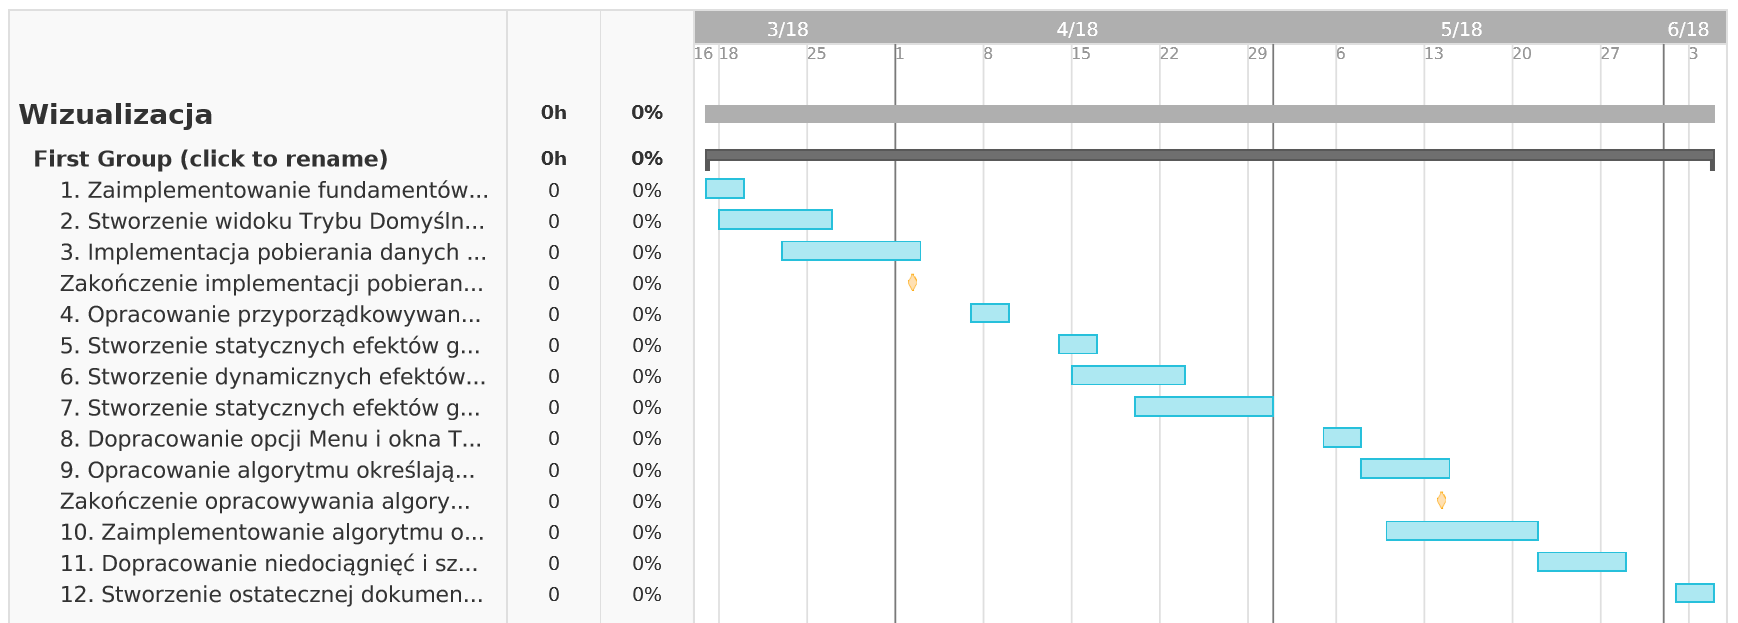
\includegraphics[width=\linewidth]{gantt.png}
	\caption{Wykres Gantta}
	\end{figure}
\section{Projekt graficznego interfejsu użytkownika} 
	\begin{flushleft}
	Okno \textit{Trybu Domyślnego} włącza się wraz z uruchomieniem programu. Na pasku menu znajdują się trzy pozycje. \\
	\end{flushleft}
\begin{enumerate}
\item Pierwsza od lewej pozycja to opcja rozwijania listy dostępnych szczytów, posegregowana alfabetycznie. Klikając wybrany szczyt następuje przejście do okna \textit{Trybu Szczytu} z danymi pogodowymi i narciarskimi wybranej góry. Pozycja została nazwana jako zatytułowana "Szczyt". \\
\item Druga od lewej pozycja to "Aktualizacja pogody". W momencie kliknięcia tej opcji, aplikacja dokona pobrania aktualnych danych pogodowych i narciarskich z danego portalu internetowego. \\
\item Trzecia pozycja od lewej, nazwana "Przełącz Widok", po kliknięciu w nią, ma zmienić rodzaj mapy z graficznej na geograficzną i z powrotem.  \\
\end{enumerate}
	\begin{flushleft}
	Niżej, pod paskiem menu, znajdować się będzie mapa południowej Polski z zaznaczonymi lokalizacjami kilku szczytów. Wokół lokalizacji danego szczytu znajdą się następujące grafiki:\\
	\end{flushleft}
	\begin{enumerate}
\item Pierwszą grafiką jest symbol pogodowy, który będzie reprezentował klasycznymi symbolami meteorologicznymi pokazywał zachmurzenie i opady w tym rejonie. \\
\item Druga pozycja to wartość średniej temperatury w ciągu dnia. \\
\item Trzecia grafika będzie reprezentować poziom pokrywy śnieżnej. W zależności od danej grubości warstwy śniegu będzie przedstawiała wzgórze o odpowiedniej ilości placów śniegu. \\
\item Obok góry na mapie znajdować się będzie jej nazwa. \\
\item Ostatnią pozycją graficzną będzie lokalizacja szczytu. Otoczona będzie kolorowym kręgiem, który będzie przedstawiał ogólny stan warunków narciarskich na tej górze. Czerwony kolor oznacza fatalny stan, gdy zielony reprezentuje idealne warunki narciarskie. Przy najechaniu myszką na tę pozycję wyświetli bardziej szczegółowa lista ocenianych kategorii, która wpłynęła na ostateczny wynik oceny szczytu. Kliknięcie lokalizacji szczytu zaowocuje otwarciem okna okna \textit{Trybu Szczytu} z danymi pogodowymi i narciarskimi wybranej góry.\\
\end{enumerate}
\begin{flushleft}
	Okno \textit{Trybu Szczytu} można uruchomić z okna \textit{Trybu Domyślnego} poprzez klikniecie szczytu z rozwijanej listy lub poprzez kliknięcie lokalizacji szczytu na mapie. Na pasku menu będzie tylko wyświetlona nazwa wybranego szczytu po lewej oraz opcja powrotu do widoku \textit{Trybu Domyślnego}. 
	Lewa strona okna będzie dysponować danymi warunków pogodowych. Prawa strona przedstawiać będzie warunki narciarskie.\\
		\end{flushleft}
	\begin{enumerate}
\item Pierwszą grafiką w warunkach narciarskich jest symbol pogodowy, który będzie reprezentował klasycznymi symbolami meteorologicznymi zachmurzenie i opady w tym rejonie. \\
\item Obok umieszczone zostaną wartości temperatury za dnia i nocy. \\
\item Poniżej zamieszczone zostaną dane o ciśnieniu atmosferycznym, prędkości wiatru oraz godzinie wschodu i zachodu słońca. \\
\item W warunkach narciarskich będzie w pierwszej kolejności przedstawiony poziom opadów śnieżnych. Napisana zostanie ilość cm grubości warstwy śniegu oraz data ostatnich opadów. Obok zamieszczona będzie grafika reprezentującą stan ośnieżenia stoku. \\
\item Drugą informacją z warunków narciarskich będzie ilość czynnych wyciągów na stokach tej góry. Obok znajdować się będzie grafika reprezentująca właśnie tę wartość.\\
\item Ostatni element graficzny będzie związany z oceną stanu pogodowego i narciarskiego wzgórza. Za pomocą odpowiedniego algorytmu, aplikacja będzie podsumowywała wszystkie parametry danego wzgórza i wystawiać ocenę w skali 1--5. Ocena będzie też reprezentowana przez krążek o różnych kolorach. Czerwień będzie odpowiadał ocenie 1, pomarańcz ocenie 2, żółty ocenie 3, limonkowy ocenie 4 i zieleń ocenie 5.\\
\end{enumerate}


\begin{flushleft}
	\end{flushleft}
	\begin{figure}[h]
	\centering
	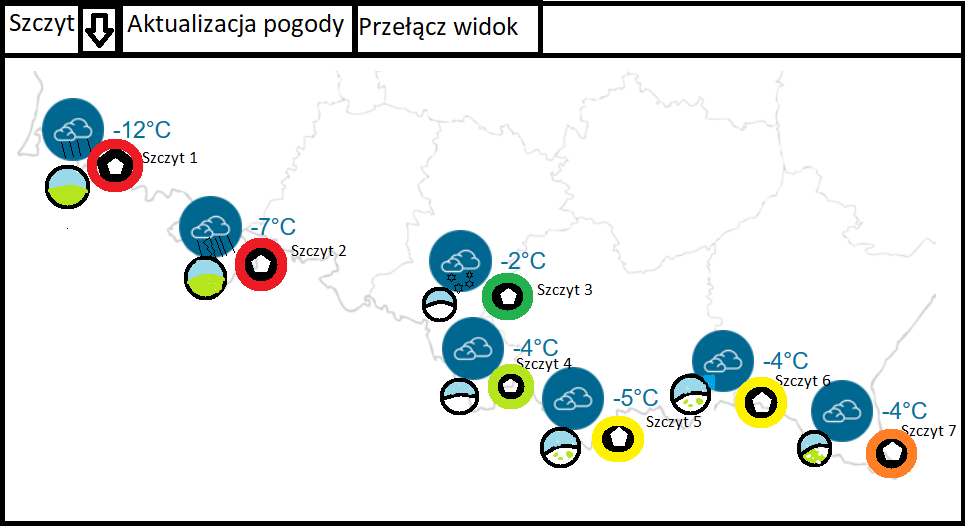
\includegraphics[width=\linewidth]{menu2.png}
	\caption{Tryb Domyślny}
	\end{figure}
	
	\begin{figure}[h]
	\centering
	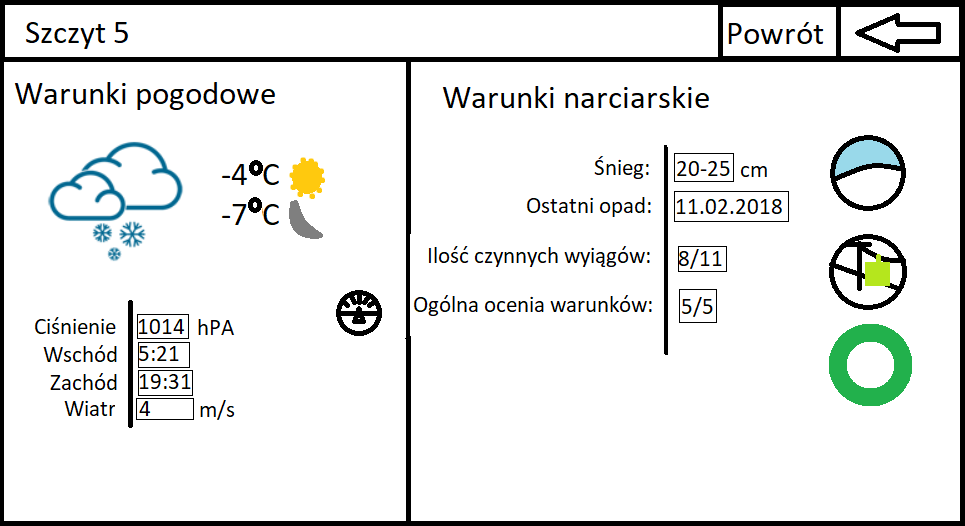
\includegraphics[width=\linewidth]{szczytu.png}
	\caption{Tryb Szczytu}
	\end{figure}
\newpage
\addcontentsline{toc}{section}{Bibilografia}
\bibliography{bibliografia}
\bibliographystyle{plain}


\end{document}







































